\section{Auswertung zum Shinriki-Oszillator}

\subsection{Phasendiagramm}
Im Folgenden wurde ein Phasendiagramm des Shinrinki-Oszillators mit den Werten \(R_1\) und \(R_2\) erstellt. Dafür wurden Schnittpunkte der Phasenübergänge ermittelt und mithilfe eines Python-Skripts wurde diese Punkte mit einer Funktion verbunden. Daraus ergibt sich folgende Abbildung, welche die Übergänge der verschiedenen Phasen abhängig von den Werten der Widerstände darstellen. Jede Line stellt dabei einen Phasenübergang dar.

\begin{figure}[h]
    \centering
    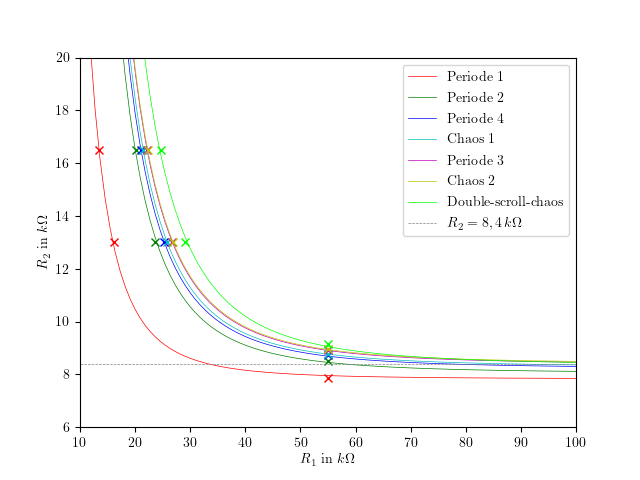
\includegraphics[scale=0.75]{AuswPaul/PhasendiagrammFertig.png}
    \label{fig:Phasendiagramm}
    \caption{Phasendiagramm}
\end{figure}

Die Funktion welche benutzt wurde, um die Punkte zu verbinden ist:
\begin{align}
    f = \frac{a}{x^3} +b
\end{align}

Diese Funktion wurde ausgewählt, indem mehrere verschiedene Funktionen ausprobiert wurden. Nachfolgend ausgewählte Funktionen zum Vergleich, um die Auswahl nachvollziehen zu können.
\begin{figure}[h]

    \centering
    
    \begin{subfigure}[b]{0.45\textwidth}
        \centering
        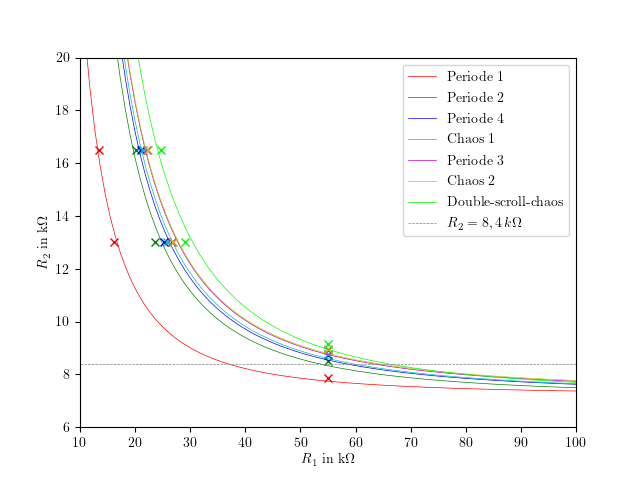
\includegraphics[width=\textwidth]{AuswPaul/PhaDiaGrad-2.png}
        \caption{$f = \frac{a}{x^2} + b$}
    \end{subfigure}
    \hfill
    \begin{subfigure}[b]{0.45\textwidth}
        \centering
        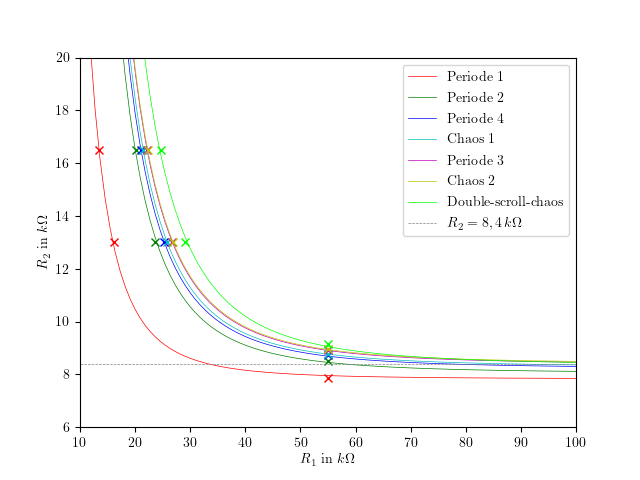
\includegraphics[width=\textwidth]{AuswPaul/PhasendiagrammFertig.png}
        \caption{$f = \frac{a}{x^3} + b$}
    \end{subfigure}
    \\
    \begin{subfigure}[b]{0.45\textwidth}
        \centering
        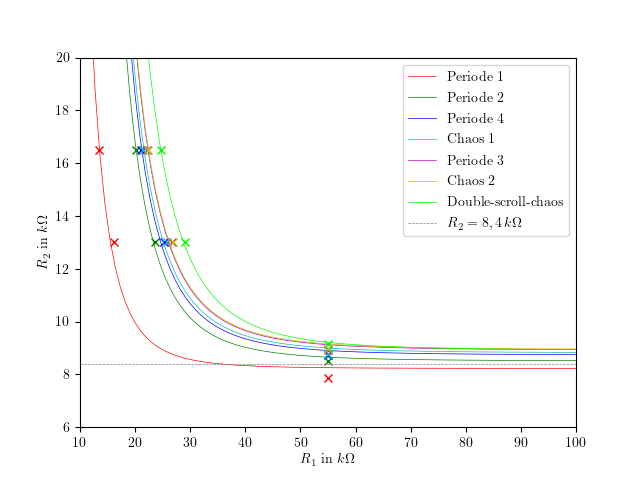
\includegraphics[width=\textwidth]{AuswPaul/PhaDiaGrad-4.png}
        \caption{$f = \frac{a}{x^4} + b$}
    \end{subfigure}
    \caption{Vergleich verschiedener 'Fitting'-Funktionen}
    \label{fig:PhasenDiaVergl}
    \end{figure}\\
\newpage
Anbei noch die errechneten Parameter für die einzelnen Funktionen: \\
\begin{table}[h]
    \centering
    \begin{tabular}{l|r|r}
            Übergang auf &          a &     b \\
            \hline
               Periode 1 &   21098,64 &  7,83 \\
               Periode 2 &   67878,80 &  8,05 \\
               Periode 4 &   77374,66 &  8,23 \\
                 Chaos 1 &   81341,62 &  8,28 \\
               Periode 3 &   88743,91 &  8,37 \\
                 Chaos 2 &   89540,79 &  8,40 \\
     Double-scroll-chaos &  119710,19 &  8,33 \\
    \end{tabular}
    \caption{Fitting-Parameter}
\end{table}



\subsection{Schnitt durch das Phasendiagramm}
Nun wird für einen festen Wert (\(R_2 = 8,4 k\Omega\)) ein Schnitt durch das Phasendiagramm erzeugt, indem \(R_1\) variiert wird und die Veränderungen aufmerksam beobachtet werden. \\
Im Folgenden unsere Beobachtungen bei ausgewählten Werten von \(R_1\).\\

\begin{figure}[h]
    \centering
    \begin{subfigure}[b]{0.45\textwidth}
        \centering
        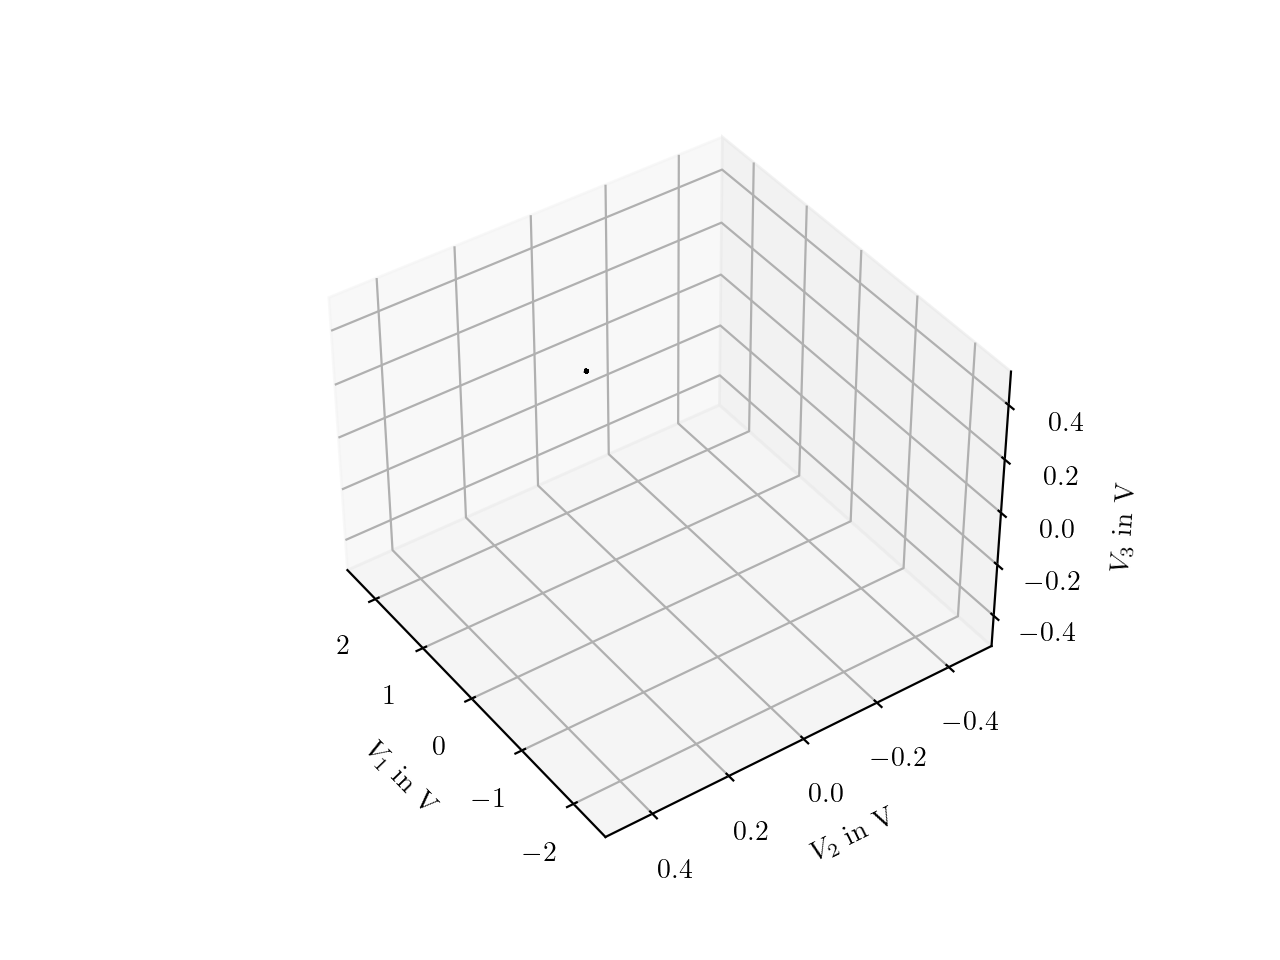
\includegraphics[width=\textwidth]{AuswPaul/Aufg-b/At37.png}
        \caption{Atraktor}
    \end{subfigure}
    \hfill
    \begin{subfigure}[b]{0.45\textwidth}
        \centering
        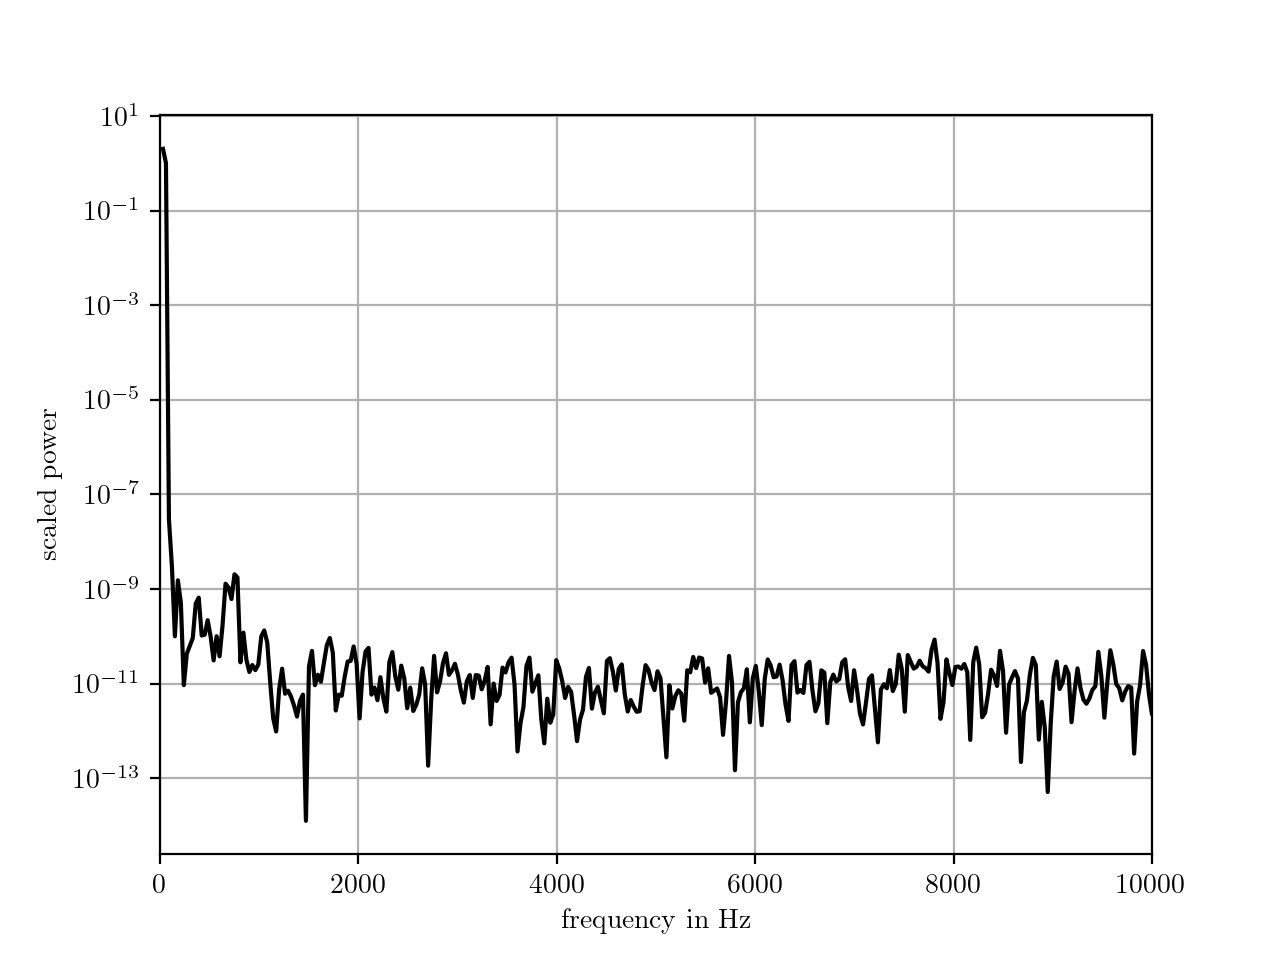
\includegraphics[width=\textwidth]{AuswPaul/Aufg-b/LS37.png}
        \caption{Leistungsspektrum}
    \end{subfigure}
    \caption{$R_1 = 37$ k$\Omega$}
\end{figure}

Bei $R_1 = 37$ k$\Omega$ ist anhand des Attraktors zu erkennen, dass keine Schwingung auftritt. Auch das Leistungsspektrum verläuft, bis auf einen Peak bei ca. 0 Hz erstaunlich gleichmäßig und bis auf Störungsrauschen nahezu horizontal. Dies spricht ebenfalls für ein schwingungsfreies System.\\

\begin{figure}[h]
    \centering
    \begin{subfigure}[b]{0.45\textwidth}
        \centering
        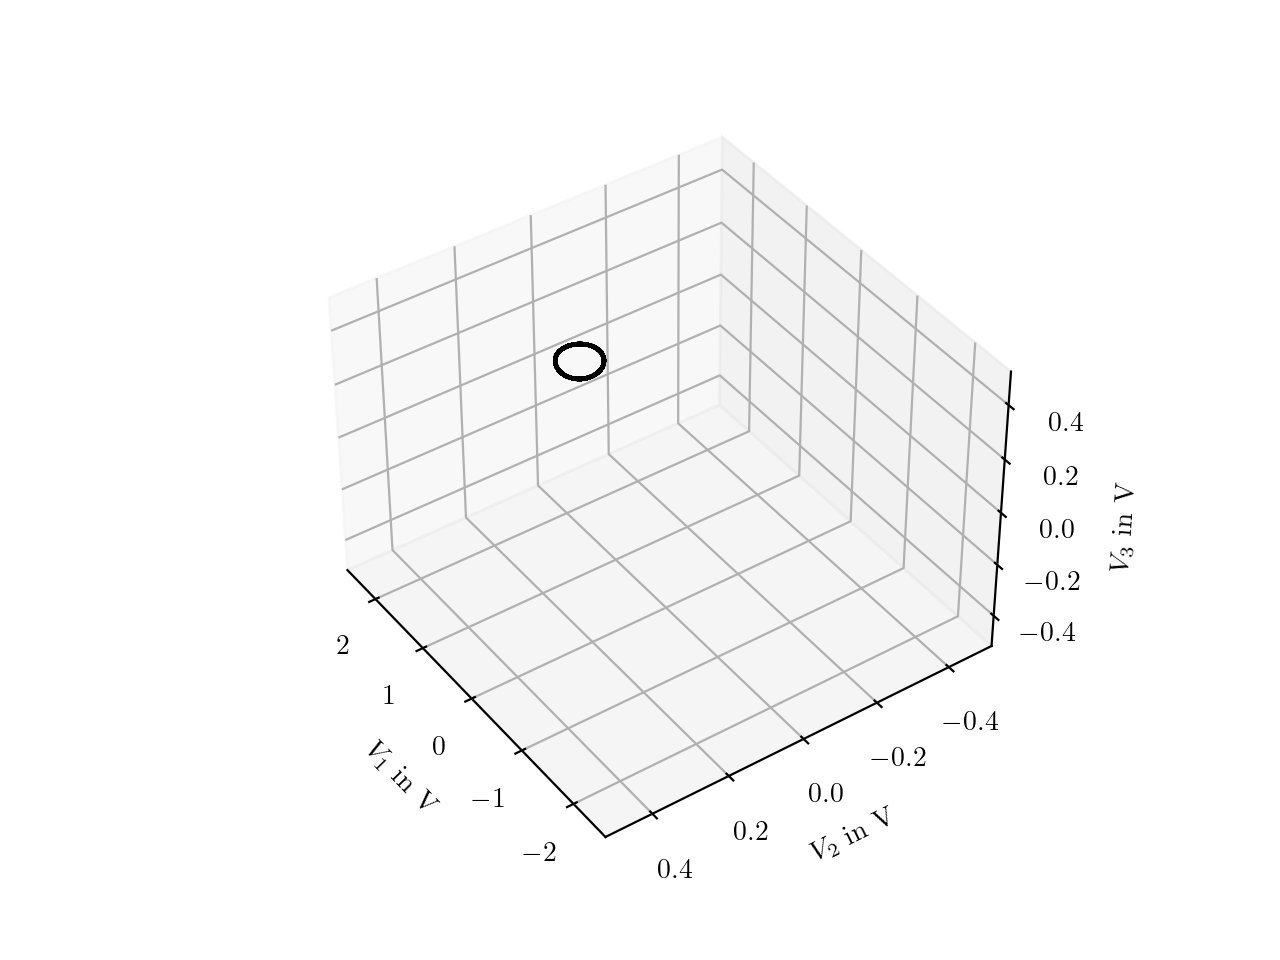
\includegraphics[width=\textwidth]{AuswPaul/Aufg-b/At40.png}
        \caption{Atraktor}
    \end{subfigure}
    \hfill
    \begin{subfigure}[b]{0.45\textwidth}
        \centering
        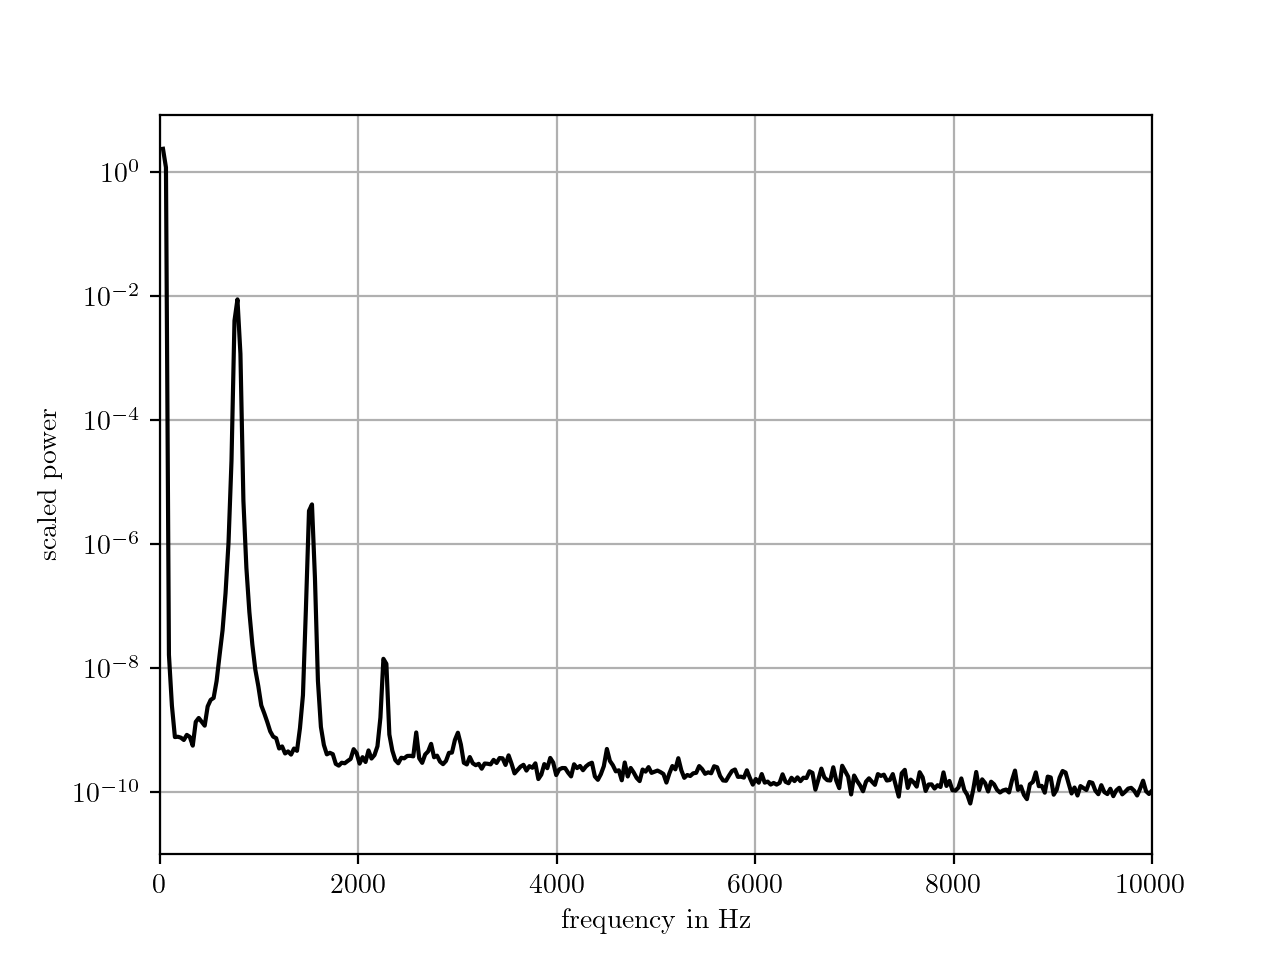
\includegraphics[width=\textwidth]{AuswPaul/Aufg-b/LS40.png}
        \caption{Leistungsspektrum}
    \end{subfigure}
    \caption{$R_1 = 40$ k$\Omega$}
\end{figure}

Für $R_1 =40$ k$\Omega$ befindet sich der Shinriki-Oszilator bereits in Periode 1, was deutlich anhand des Attraktors zu erkennen ist. Auch im Leistungsspektrum sind nun deutliche Unterschiede im Vergleich zum vaorrangegangenen zu erkennen. Es existieren nun mehrere Peaks.

\begin{figure}[h]
    \centering
    \begin{subfigure}[b]{0.45\textwidth}
        \centering
        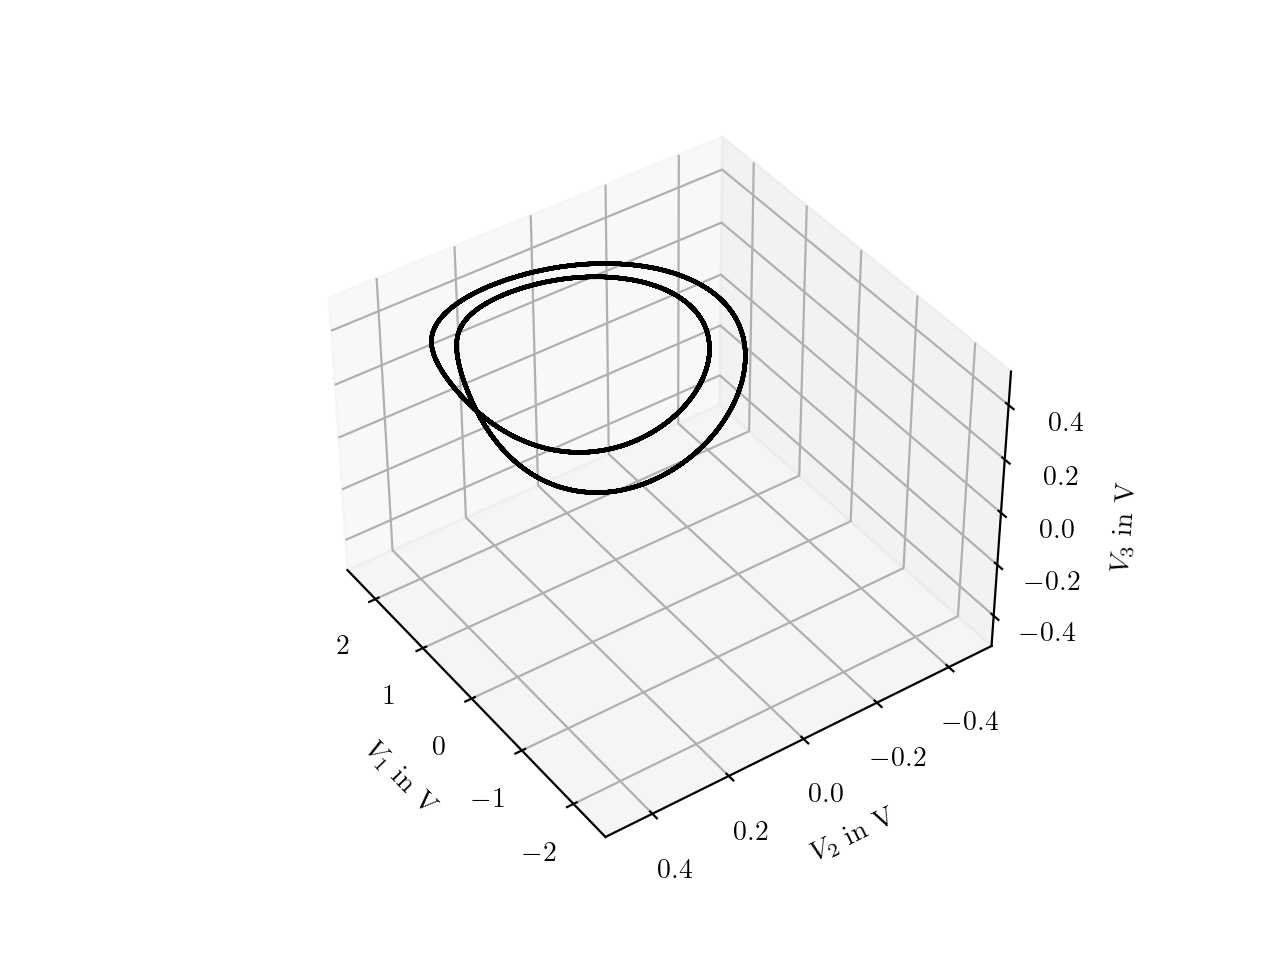
\includegraphics[width=\textwidth]{AuswPaul/Aufg-b/At60.png}
        \caption{Atraktor}
    \end{subfigure}
    \hfill
    \begin{subfigure}[b]{0.45\textwidth}
        \centering
        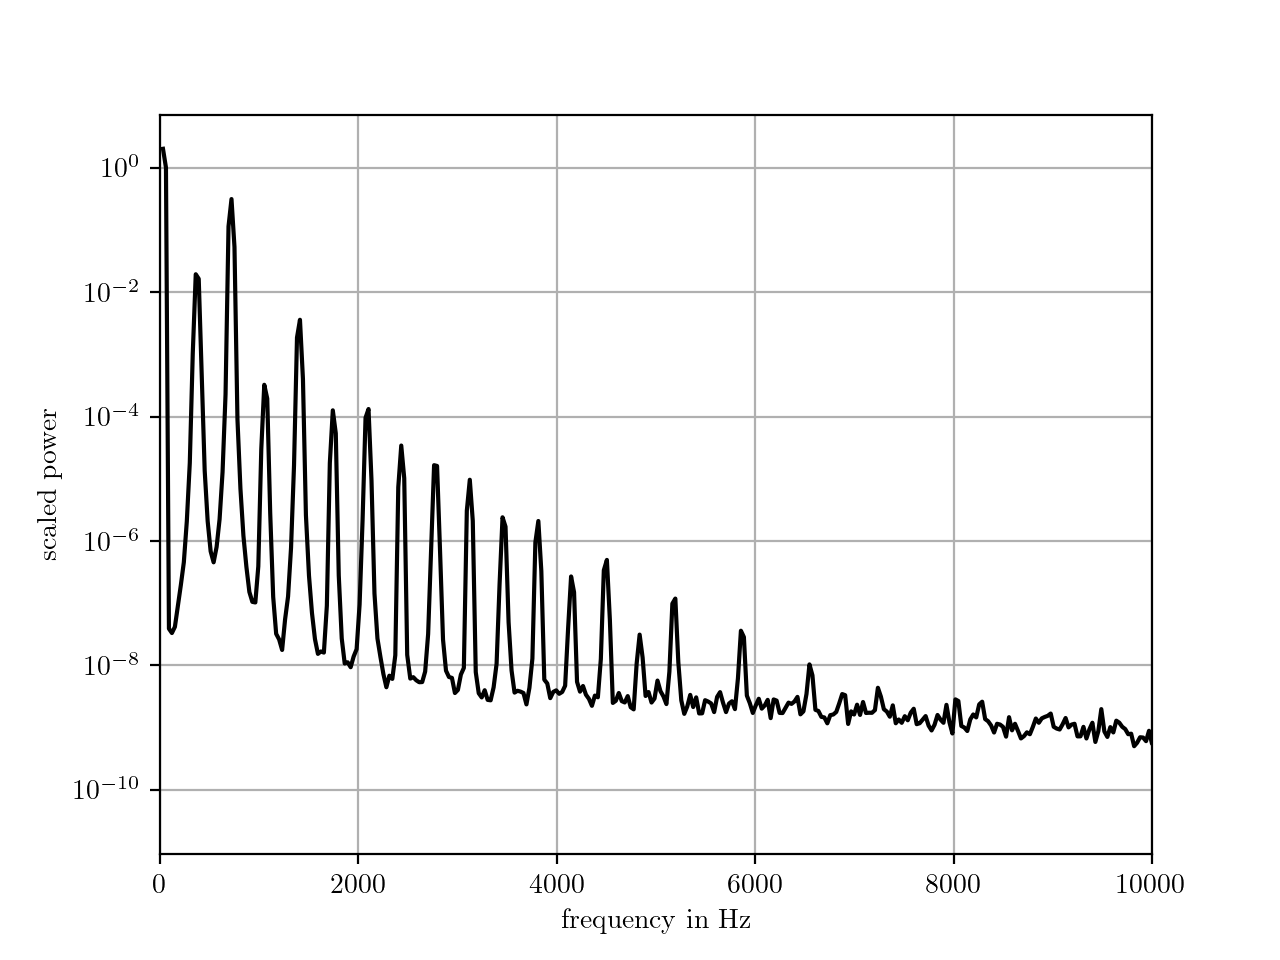
\includegraphics[width=\textwidth]{AuswPaul/Aufg-b/LS60.png}
        \caption{Leistungsspektrum}
    \end{subfigure}
    \caption{$R_1 = 60$ k$\Omega$}
\end{figure}

Eine deutliche Zunahme an Peaks ist bei $R_1 = 60$ k$\Omega$ zu erkennen. Anhand des Attraktors ist sehr gut zu erkennen, dass es sich nun um Periode 2 handelt. Im Vergleich zum letzten Mal fand also ein Bifurkation statt.

\begin{figure}[h]
    \centering
    \begin{subfigure}[b]{0.45\textwidth}
        \centering
        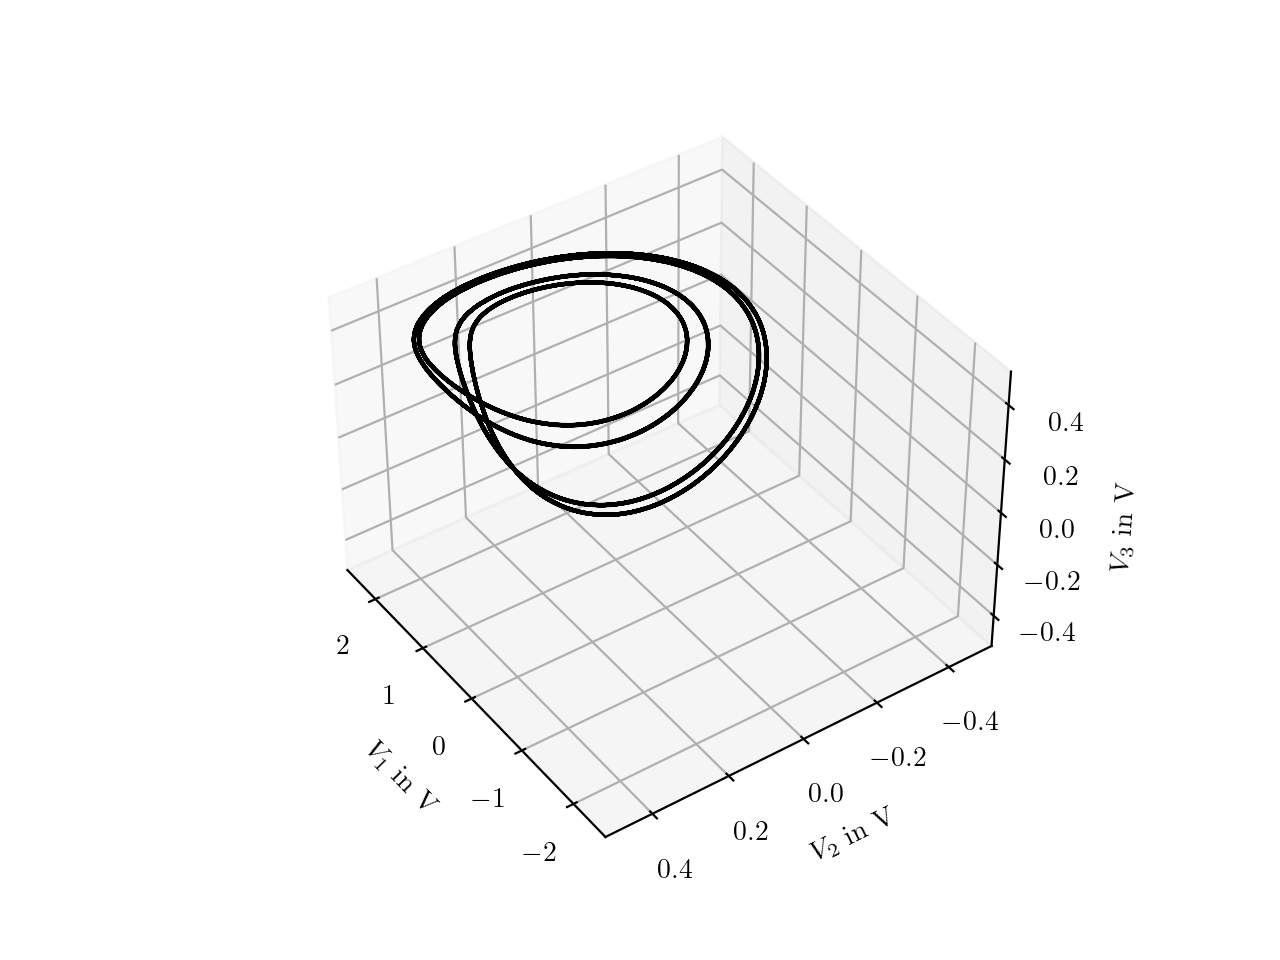
\includegraphics[width=\textwidth]{AuswPaul/Aufg-b/At66.png}
        \caption{Atraktor}
    \end{subfigure}
    \hfill
    \begin{subfigure}[b]{0.45\textwidth}
        \centering
        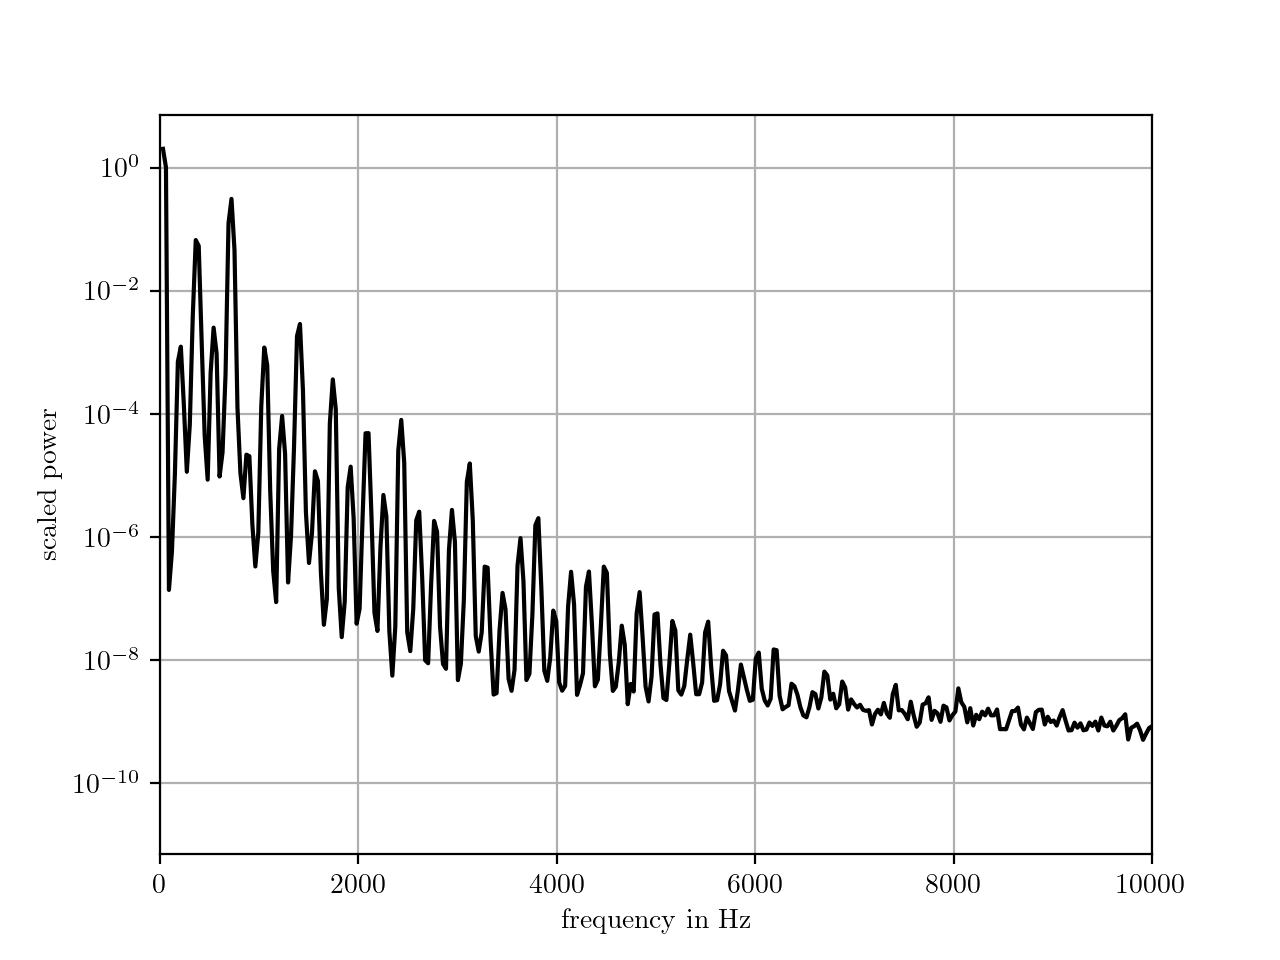
\includegraphics[width=\textwidth]{AuswPaul/Aufg-b/LS66.png}
        \caption{Leistungsspektrum}
    \end{subfigure}
    \caption{$R_1 = 66$ k$\Omega$}
\end{figure}

Eine weitere Bifurkation findet im Übergang zu $R_1 = 66$ k$\Omega$ statt. Was wiederrum durch eine Zunahme an Peaks im Leistungsspektrum begleitet wird. Ein Blick auf den Atraktor bestätigt das sich der Oszillator nun in Periode 4 befindet.
\newpage
\begin{figure}[h]
    \centering
    \begin{subfigure}[b]{0.45\textwidth}
        \centering
        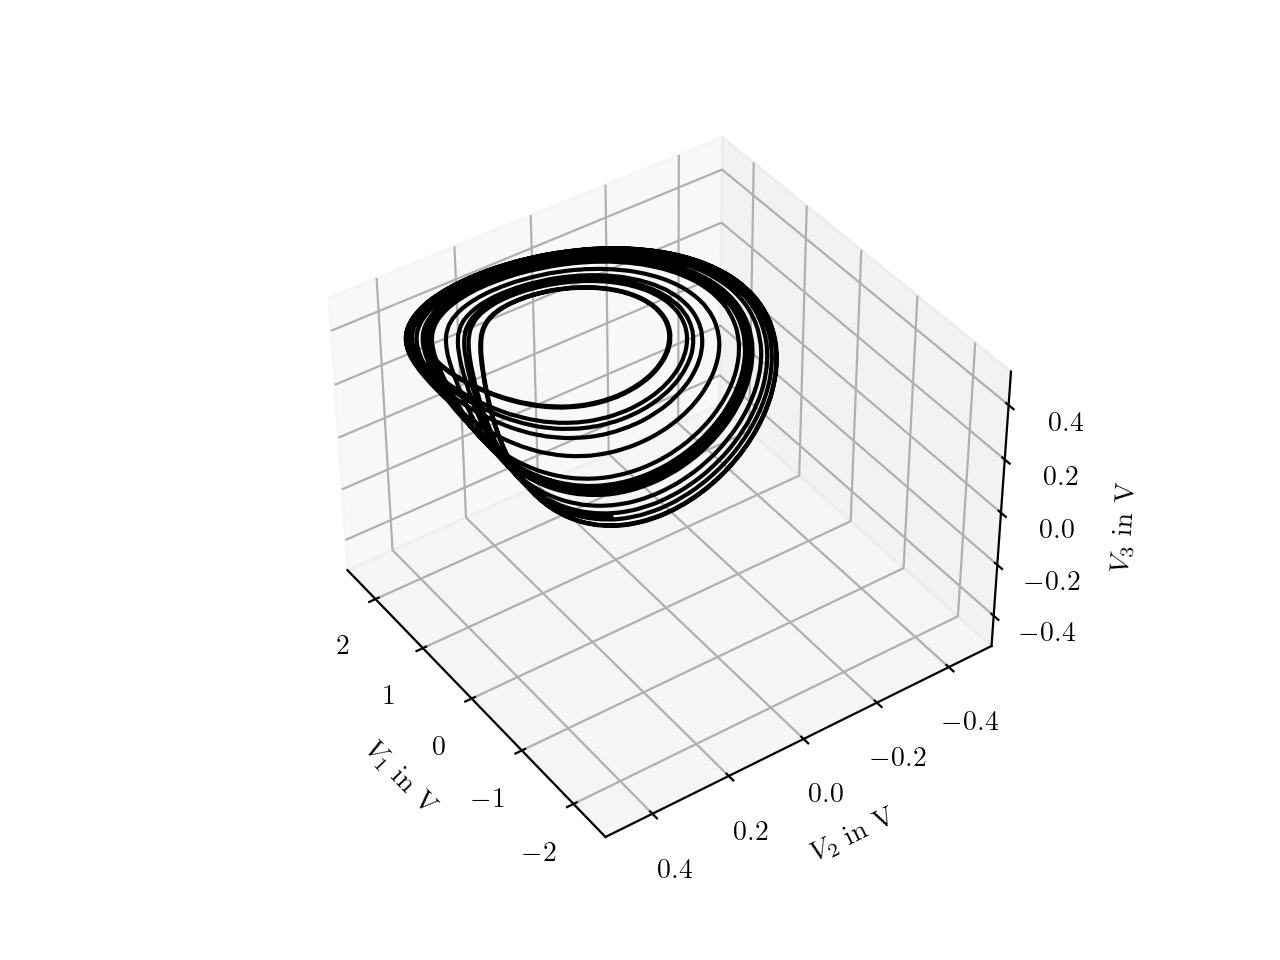
\includegraphics[width=\textwidth]{AuswPaul/Aufg-b/At70.png}
        \caption{Atraktor}
    \end{subfigure}
    \hfill
    \begin{subfigure}[b]{0.45\textwidth}
        \centering
        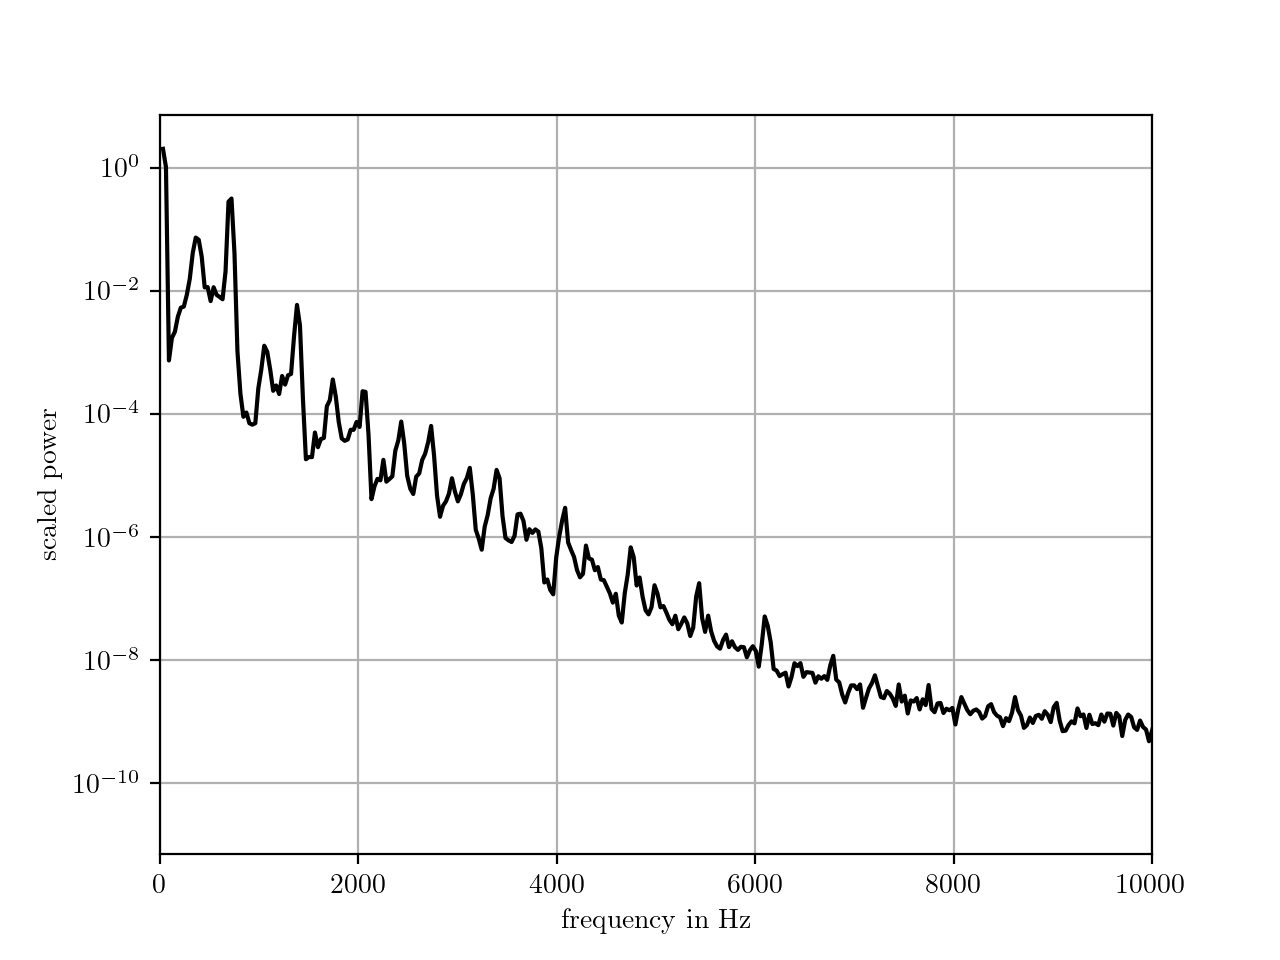
\includegraphics[width=\textwidth]{AuswPaul/Aufg-b/LS70.png}
        \caption{Leistungsspektrum}
    \end{subfigure}
    \caption{$R_1 = 70$ k$\Omega$}
\end{figure}

Die nächste Phase zeigt nun zum ersten Mal chaotisches Verhalten, was sehr gut am nahezu kontinuierlich abnehmenden Leistungsspektrum und an dem Atraktor zu erkennen ist. Dies geschieht bei $R_1 = 70$ k$\Omega$.

\begin{figure}[h]
    \centering
    \begin{subfigure}[b]{0.45\textwidth}
        \centering
        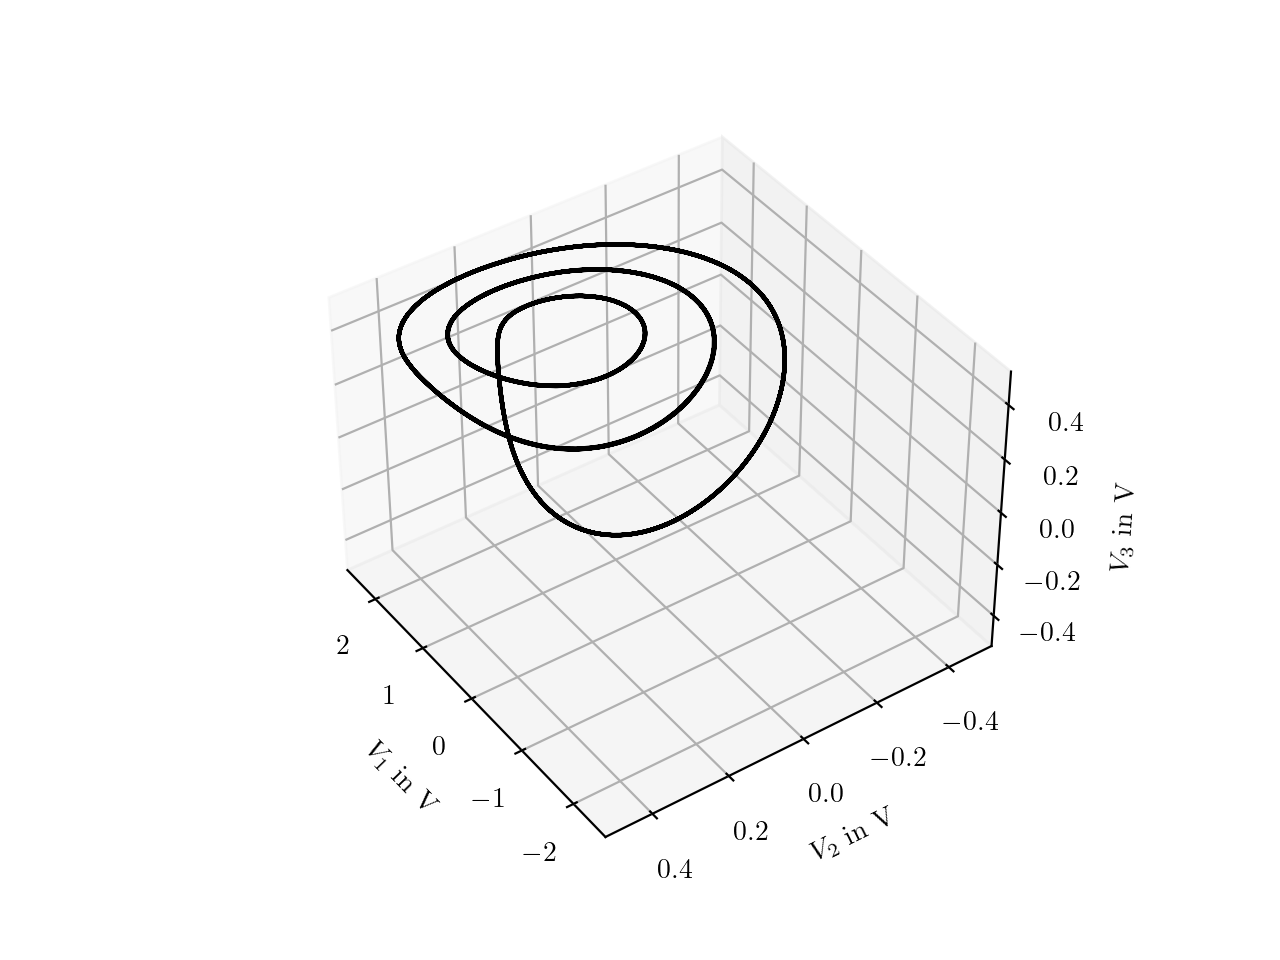
\includegraphics[width=\textwidth]{AuswPaul/Aufg-b/At73.png}
        \caption{Atraktor}
    \end{subfigure}
    \hfill
    \begin{subfigure}[b]{0.45\textwidth}
        \centering
        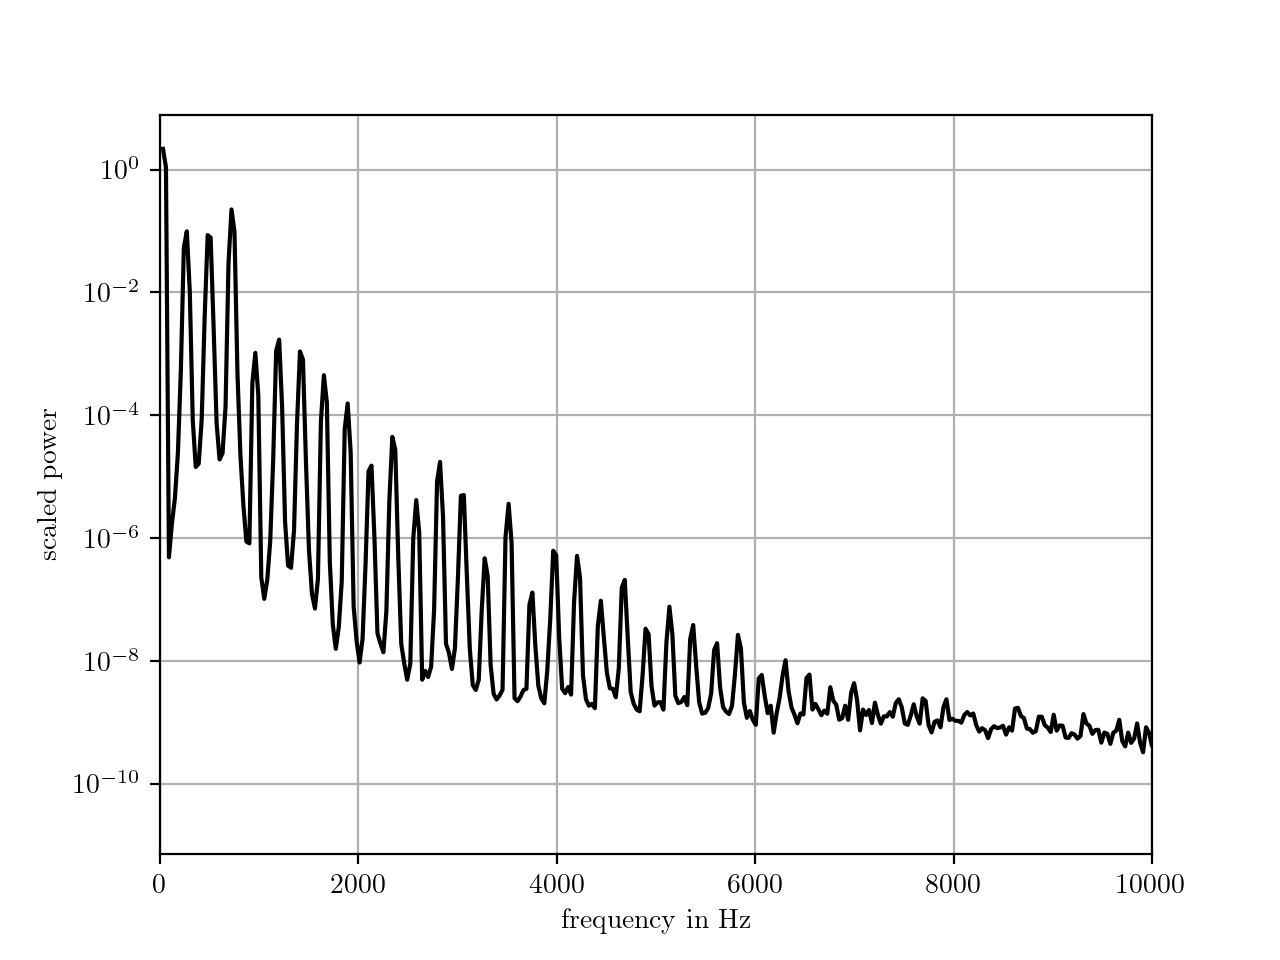
\includegraphics[width=\textwidth]{AuswPaul/Aufg-b/LS73.png}
        \caption{Leistungsspektrum}
    \end{subfigure}
    \caption{$R_1 = 73$ k$\Omega$}
\end{figure}

Das Chaos wird durch ein Periode 3 Fenster durchbrochen, was der Plot des Atraktors bei $R_1 = 73$ k$\Omega$ sehr gut verdeutlicht.

\begin{figure}[h]
    \centering
    \begin{subfigure}[b]{0.45\textwidth}
        \centering
        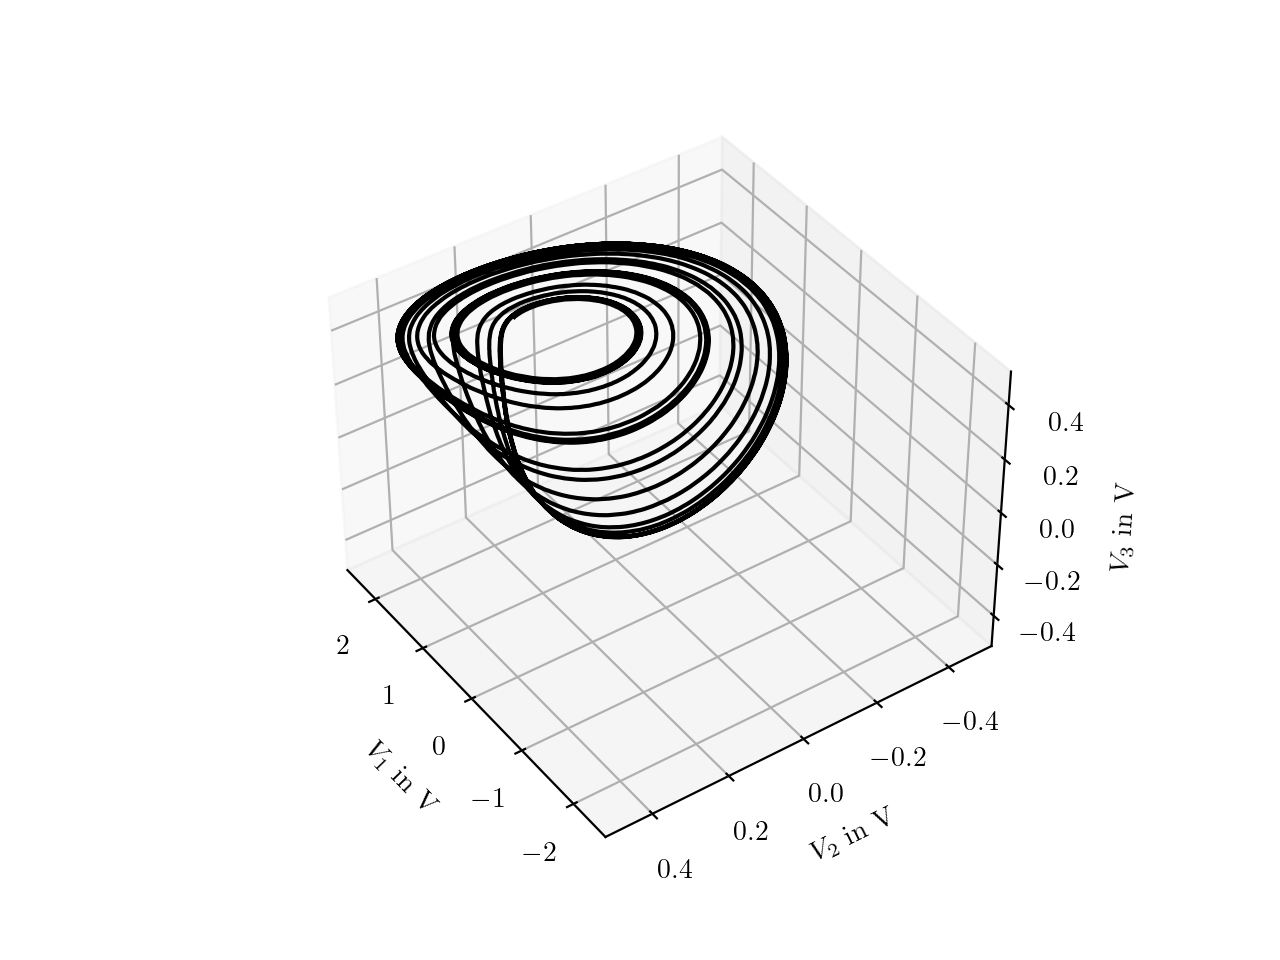
\includegraphics[width=\textwidth]{AuswPaul/Aufg-b/At74.png}
        \caption{Atraktor}
    \end{subfigure}
    \hfill
    \begin{subfigure}[b]{0.45\textwidth}
        \centering
        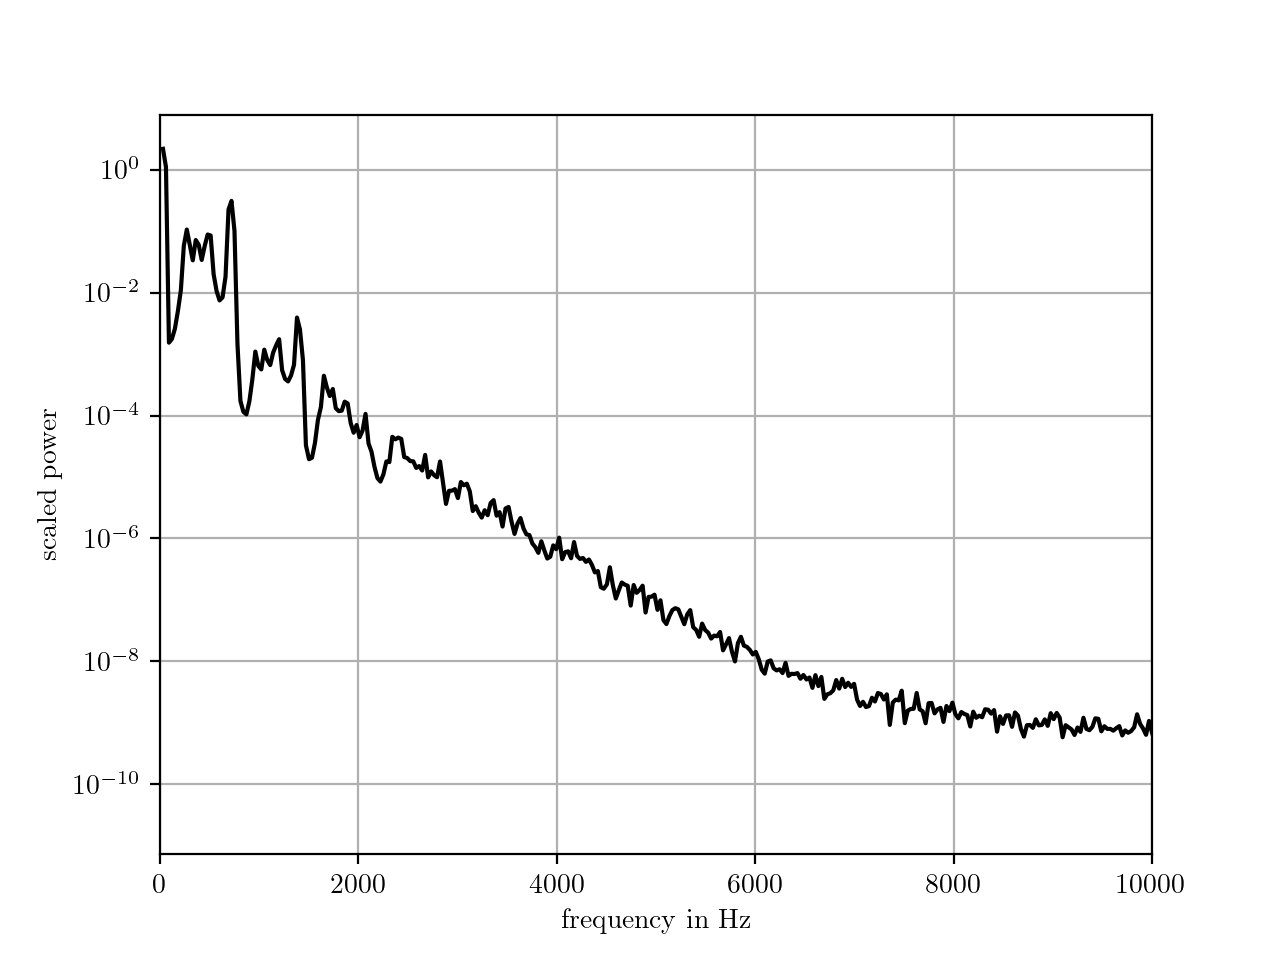
\includegraphics[width=\textwidth]{AuswPaul/Aufg-b/LS74.png}
        \caption{Leistungsspektrum}
    \end{subfigure}
    \caption{$R_1 = 74$ k$\Omega$}
\end{figure}

\newpage
Anschließend bei $R_1 = 74$ k$\Omega$ tritt, deutlich erkennbar, erneut Chaos auf.

\begin{figure}[h]
    \centering
    \begin{subfigure}[b]{0.45\textwidth}
        \centering
        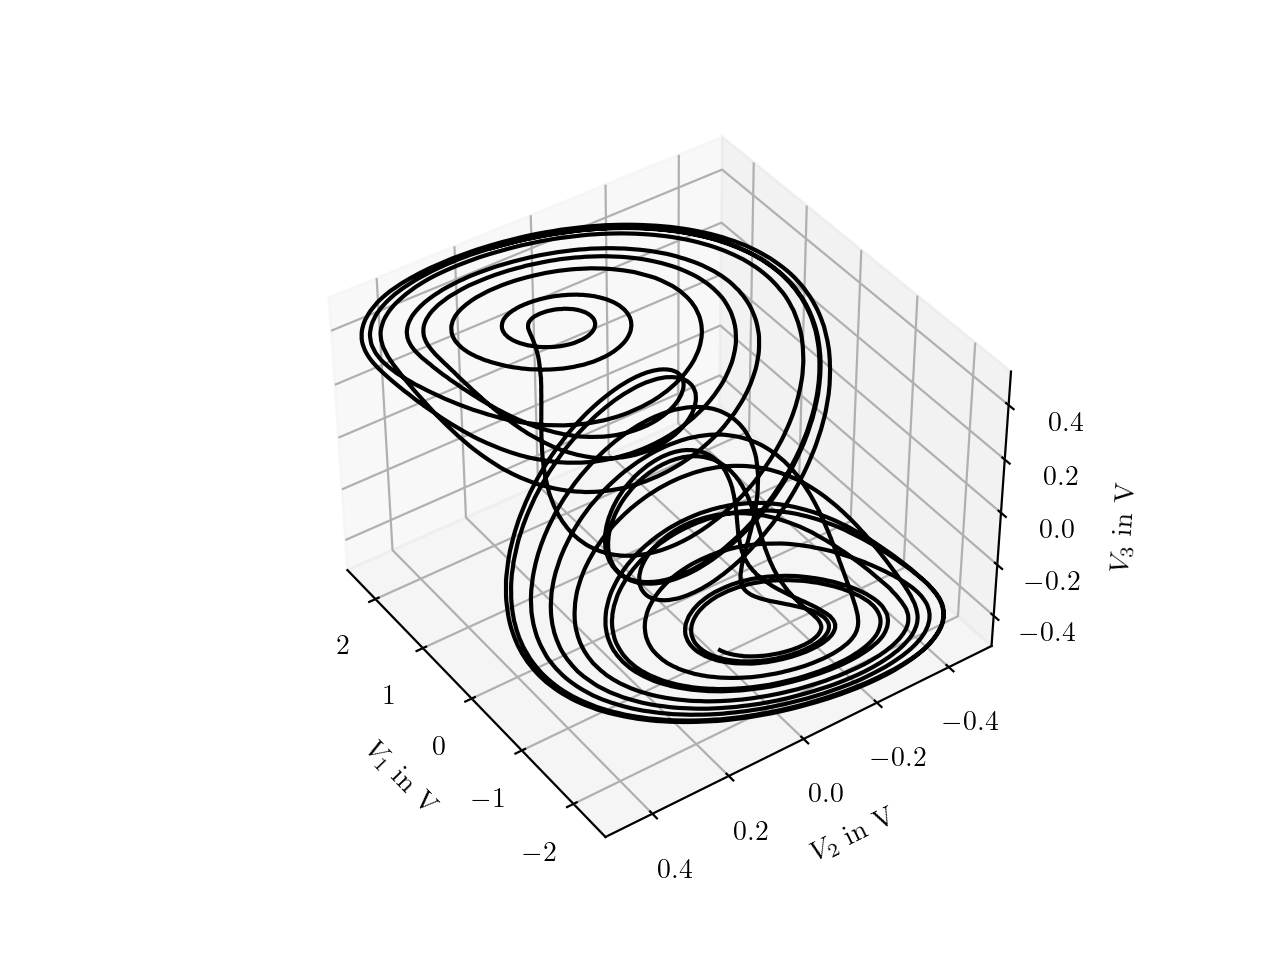
\includegraphics[width=\textwidth]{AuswPaul/Aufg-b/At100.png}
        \caption{Atraktor}
    \end{subfigure}
    \hfill
    \begin{subfigure}[b]{0.45\textwidth}
        \centering
        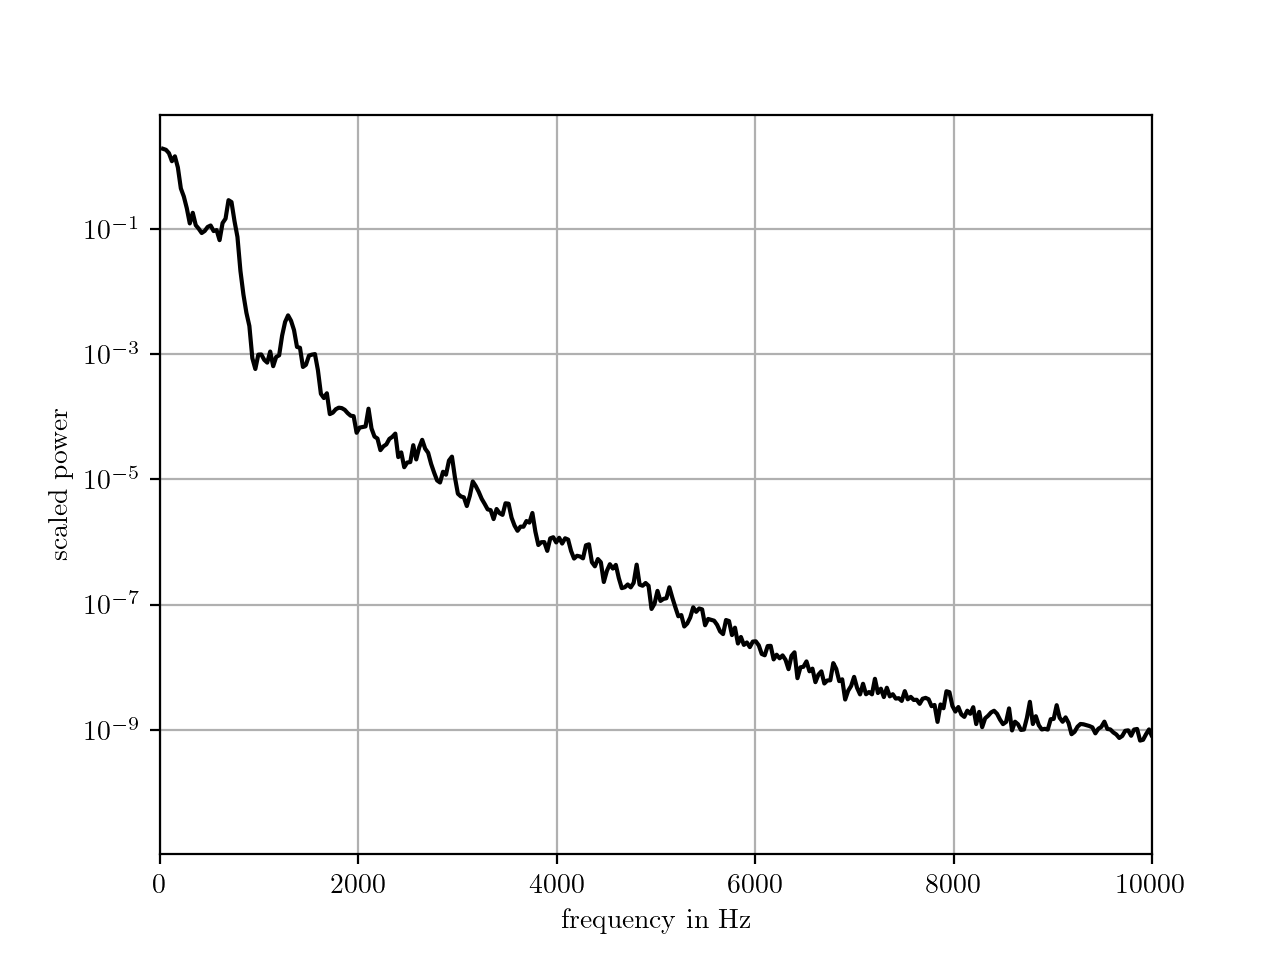
\includegraphics[width=\textwidth]{AuswPaul/Aufg-b/LS100.png}
        \caption{Leistungsspektrum}
    \end{subfigure}
    \caption{$R_1 = 100$ k$\Omega$}
\end{figure}

Bei $R_1 = 100$ k$\Omega$ ist das Double-scroll-chaos zu erkennen.
\newpage
\subsection{Bifurkationsdiagramm}
Um ein Bifurkationsdiagramm zu erstellen würde ähnlich zum Schnitt durch das Phasendiagramm ein fester Wert (\(R_2=8,4k \Omega\)) eingestellt. Unter zuhilfenahme des Labview Messprogramms konnte nun durch Variation von \(R_1\) folgendes Diagramm erstellt werden.

\begin{figure}[h]
    \centering
    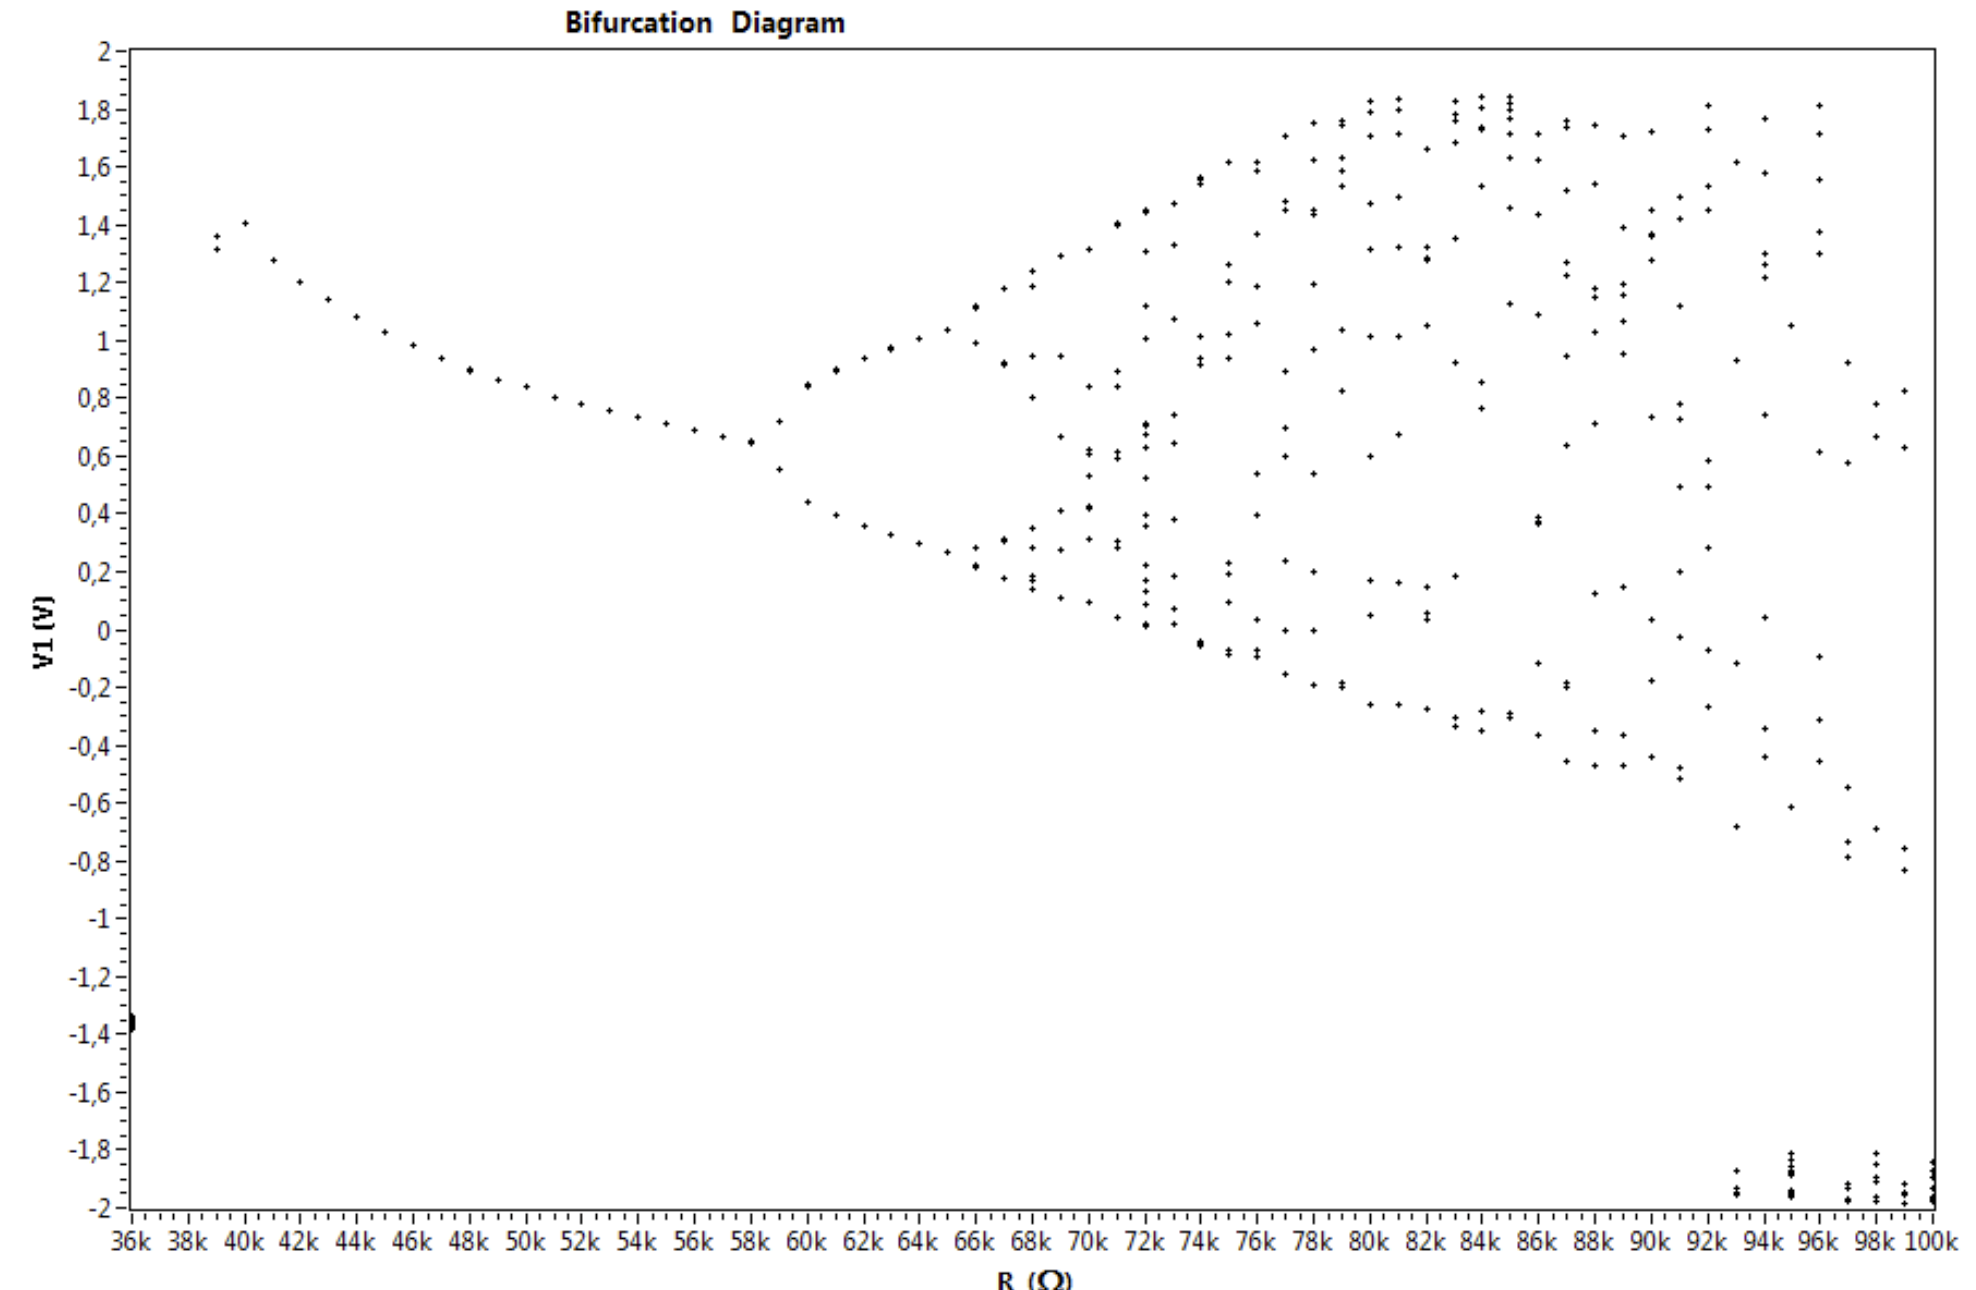
\includegraphics[width=\textwidth]{AuswPaul/BifurkDia.png}
    \caption{Bifurkationsdiagramm bei $R_2 = 8,4$ k$\Omega$ und variablen $R_1$}
\end{figure}



\subsection{Feigenbaum-Konstante}

Um die Feigenbaum-Konstante zu bestimmen wurden die Werde, bein denen eine Periodenverdopplung auftrat, ermittelt. Diese wurden durch eine separate Messung aufgenommen und nicht aus obigen Bifurkationsdiagramm abgelesen. Damit wird versucht genauere werte zu erhalten. Da für das Bifurkationsdiagramm die Messdauer, im Vergleich zum direkten Suchen der Periodenverdopplungen, deutlich größer ist, ist es wahrscheinlicher, dass Störquellen, wie Temperaturveränderungen der Messgeräte, die Werte verfälschen.\\

Die Feigenbaum-Konstante \(\delta\) kann folgendermaßen berechnet werden: 
\begin{align}
    \delta = \lim_{n \to \infty} \delta_n \\
    \delta_n = \frac{r_n - r_{n-1}}{r_{n+1} -r_n}
\end{align}

Fehlerrechnung!!\\

Der Literaturwert der Feigenbaum-Konstante ist: \(\delta = 4,6692...\)\\

Folgende Werte wurden gemessen: \\
\begin{tabular}{c c c}
    $r_1$ & $r_2$ & $r_3$\\
    \hline
    59 & 65,6 & 67,6
\end{tabular}

Mit unseren Werten ergibt sich: \(\delta_2 = (3,3 \pm ?)\)

\subsection{Zum Einbettungstheorem}